\documentclass{article}
\usepackage{graphicx}
\usepackage{fontspec}
\setmainfont{Microsoft YaHei}
\usepackage{geometry}
\setlength{\parindent}{0pt}
\usepackage{ctex}
\usepackage{algorithm}  
\usepackage{algorithmicx}  
\usepackage{algpseudocode}  
\usepackage{amsmath}  
\title{Database HW5}
\author{王嵘晟 \quad PB1711614}
\date{}
\begin{document}
	\maketitle
	\section*{ER图:}
	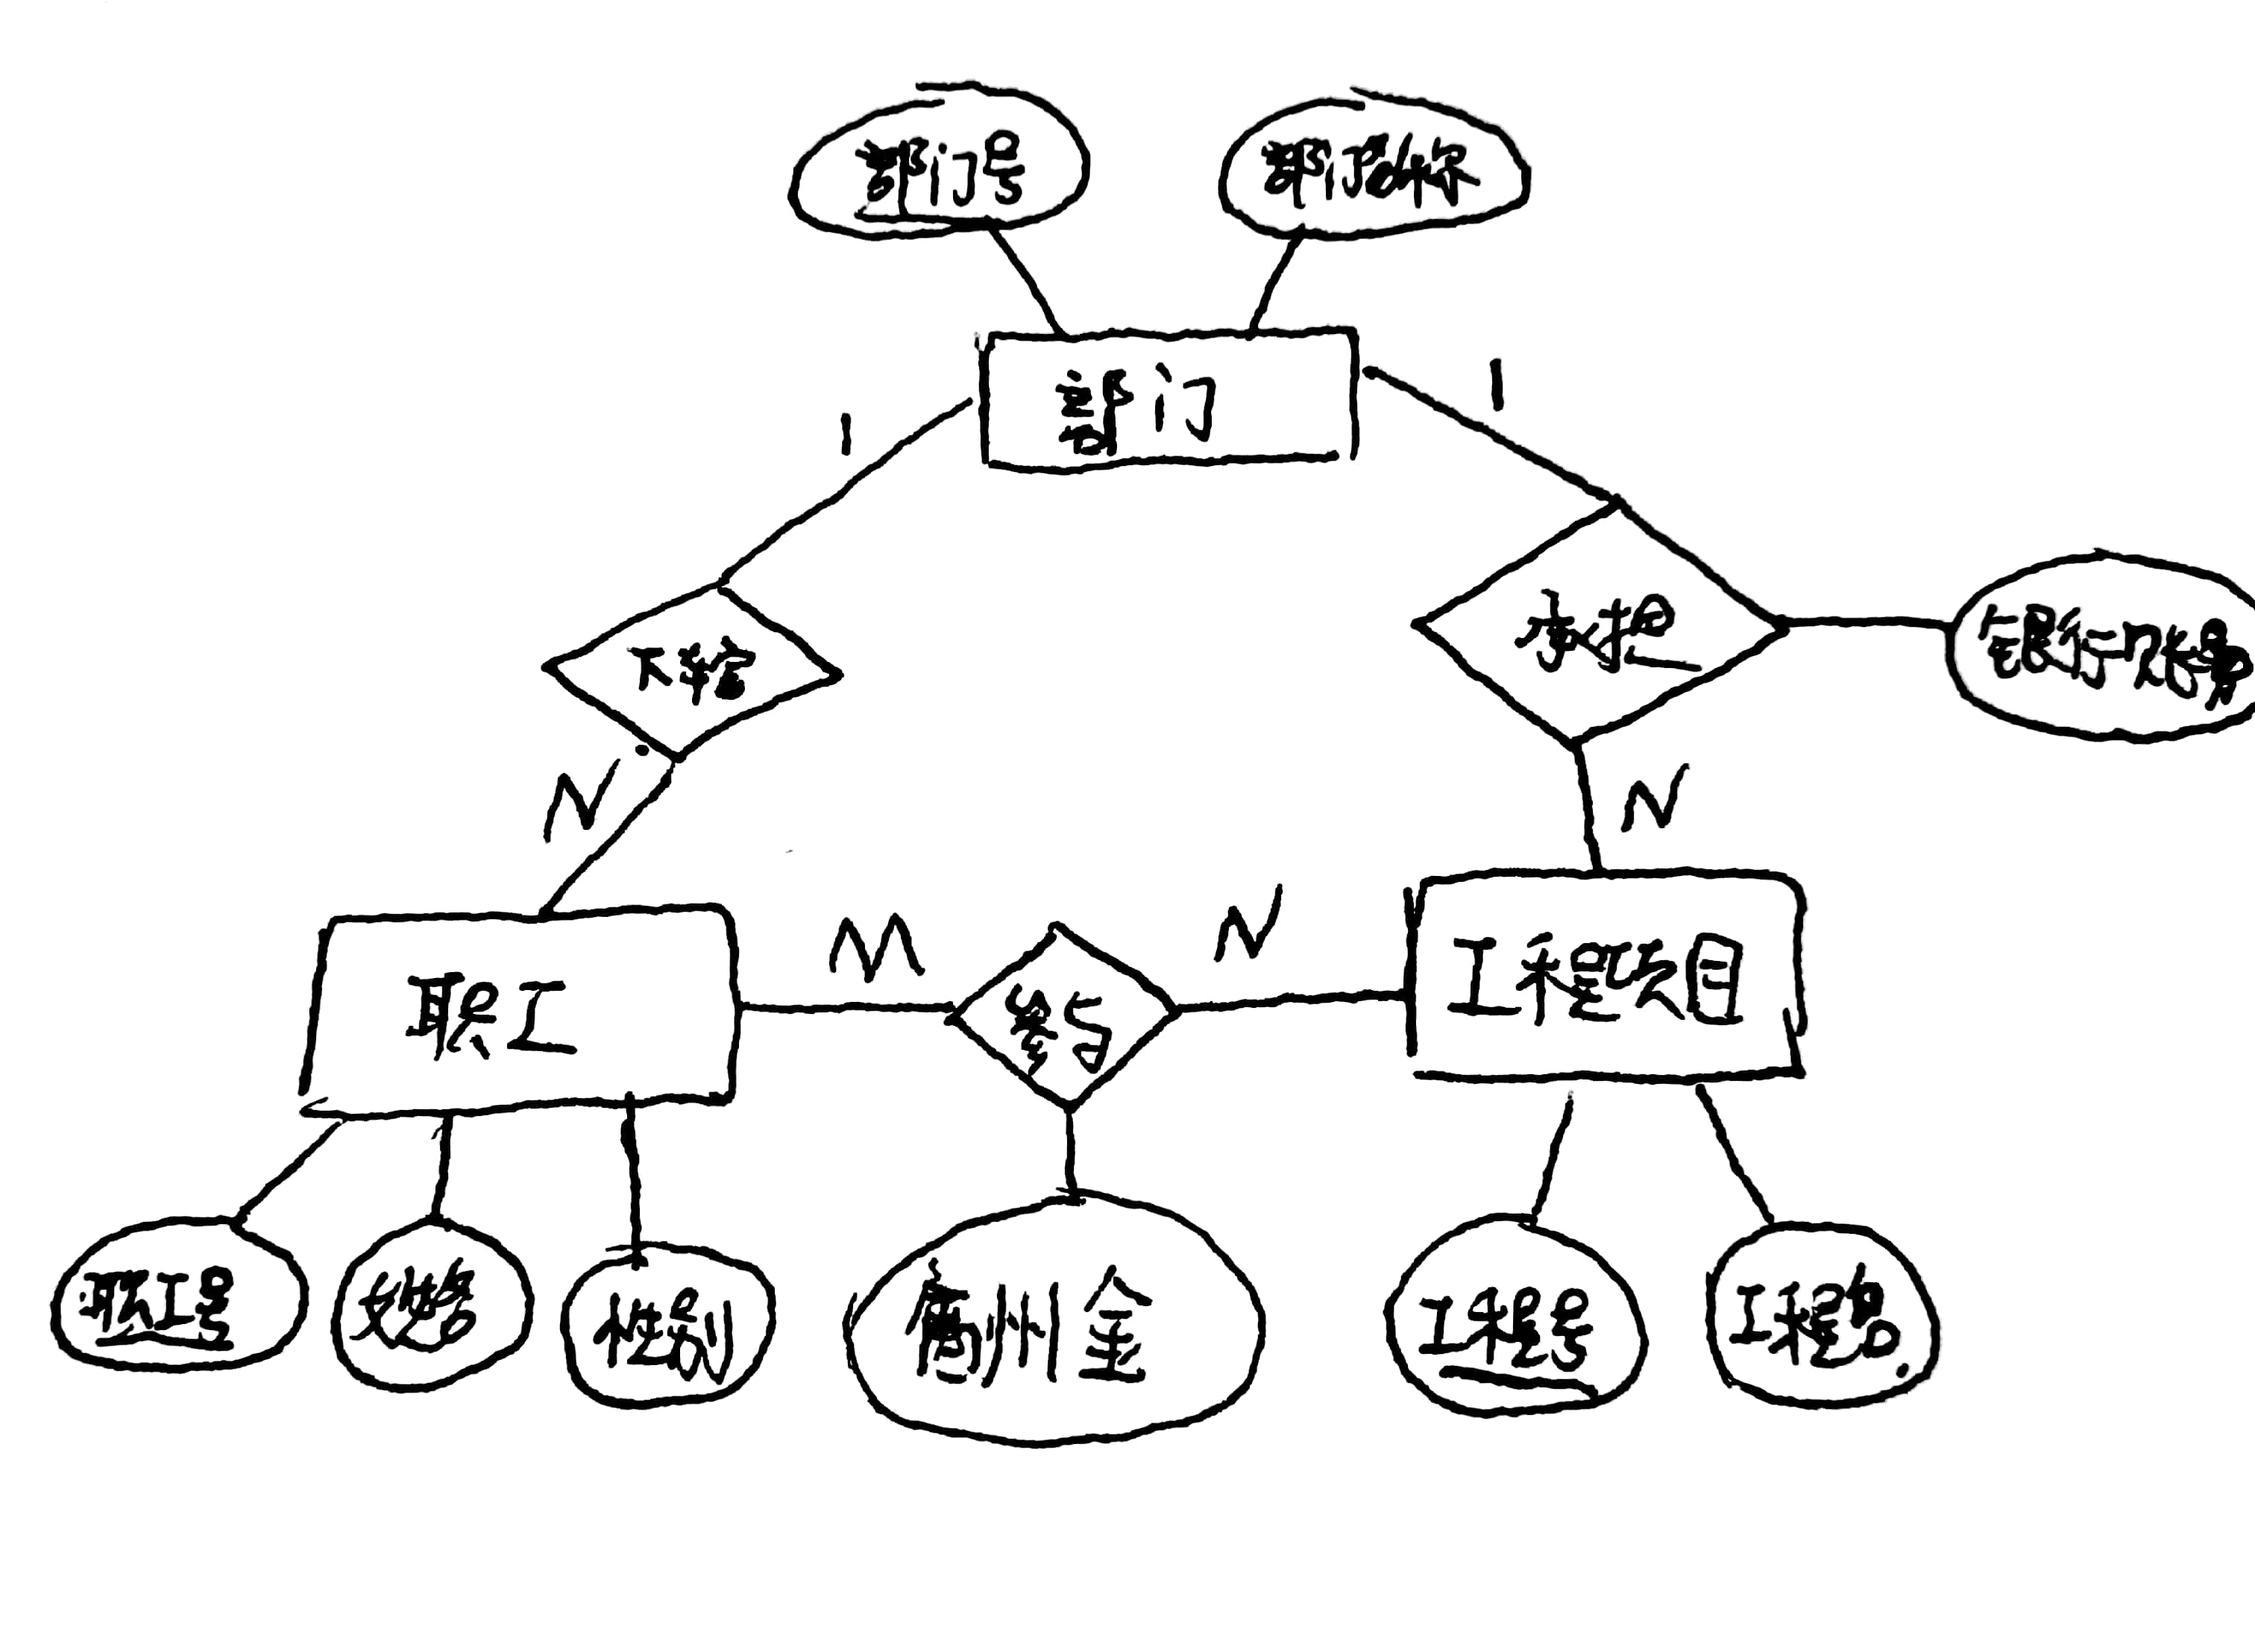
\includegraphics[scale=0.13]{2.jpg}\\
	\section*{转化成关系数据库模式:}
	\subsection*{实体转化得到关系模式:}
	$1.\ 部门(\underline{部门号},\ 部门名称)$\\
	$2.\ 职工(\underline{职工号},\ 姓名,\ 性别)$\\
	$3.\ 工程项目(\underline{工程号},\ 工程名) $
	\subsection*{考虑每个联系}
	$部门:职工(1:N)\quad 职工(\underline{职工号},\ 姓名,\ 性别,\ 部门号)$\\
	$部门:工程项目(1:N)\quad 工程项目(\underline{工程号},\ 工程名,\ 部门号,\ 银行账户)$\\
	$职工:工程项目(M:N)\quad 增加模式:\ 职工\_ 工程(\underline{职工号},\ \underline{工程号},\ 酬金)$
	\subsection*{$\textbf{最终得到关系数据模式:}$}
	$1.\ 部门(\underline{部门号},\ 部门名称)$\\
	$2.\ 职工(\underline{职工号},\ 姓名,\ 性别,\ 部门号)$\\ 
	$3.\ 工程项目(\underline{工程号},\ 工程名,\ 部门号,\ 银行账户)$\\
	$4.\ 职工\_ 工程(\underline{职工号},\ \underline{工程号},\ 酬金)$
\end{document}